\documentclass[a4paper,10pt,oneside]{article}
\usepackage[polutonikogreek,italian]{babel}
\usepackage[utf8x]{inputenc}
\usepackage{amsmath}
\usepackage{amsthm}
\usepackage{amssymb}
\usepackage{amscd}
\usepackage{graphicx}
\usepackage{float}
\usepackage{array}
\usepackage{verbatim}
\usepackage{rotating}
\usepackage[small]{caption}
\usepackage{lscape}
\usepackage{fancybox}
\usepackage{booktabs}
\parindent0ex 
\renewcommand{\fboxsep}{0.5cm}
\usepackage{hyperref}
\renewcommand{\textfraction}{0.05}
\renewcommand{\topfraction}{0.95}
\renewcommand{\bottomfraction}{0.95}
\renewcommand{\floatpagefraction}{0.35}
\setcounter{totalnumber}{5}
\restylefloat{figure}
\newlength{\drop}
\begin{document}

\begin{center}
{\huge Laboratorio di meccanica}
\end{center} 



\section{La seconda legge di Newton}


La seconda legge di Newton ci dice che se la forza $\mathbf{F}$ agisce su un corpo di massa inerziale $m$ questo acquisisce un'accelerazione $\mathbf{a}$:
\begin{equation}\label{newton_2}
 \mathbf{F}=m\mathbf{a}
\end{equation}
Dobbiamo inoltre ricordare come l'equazione (\ref{newton_2}) valga solo in sistemi di riferimento inerziali. La Terra a causa del suo moto di rotazione e rivoluzione attorno al Sole non è un sistema inerziale, la seconda legge di Newton non vale quindi rigorosamente all'interno del nostro laboratorio. Definiamo una nuova quantità che introdurremo in questo laboratorio:
\begin{equation}\label{moto}
 \mathbf{p}=m\mathbf{v}
\end{equation}
come si vede dalla (\ref{moto}) la quantità $\mathbf{p}$ è il prodotto della velocità e della massa inerziale di un corpo. Tramite questa definizione possiamo riscrivere la seconda legge della dinamica nel modo seguente:
\begin{equation}
 \mathbf{F}=\frac{d\mathbf{p}}{dt}
\end{equation}
\begin{equation}
 \mathbf{F}_m=\frac{\Delta \mathbf{p}}{\Delta t}
\end{equation}
la forza esercitata su un corpo è quindi equivalente alla variazione della sua quantità di moto, notiamo che questa varia sia se cambia la velocità del corpo sia se varia la sua massa.

\begin{figure}[H]
 \centering
 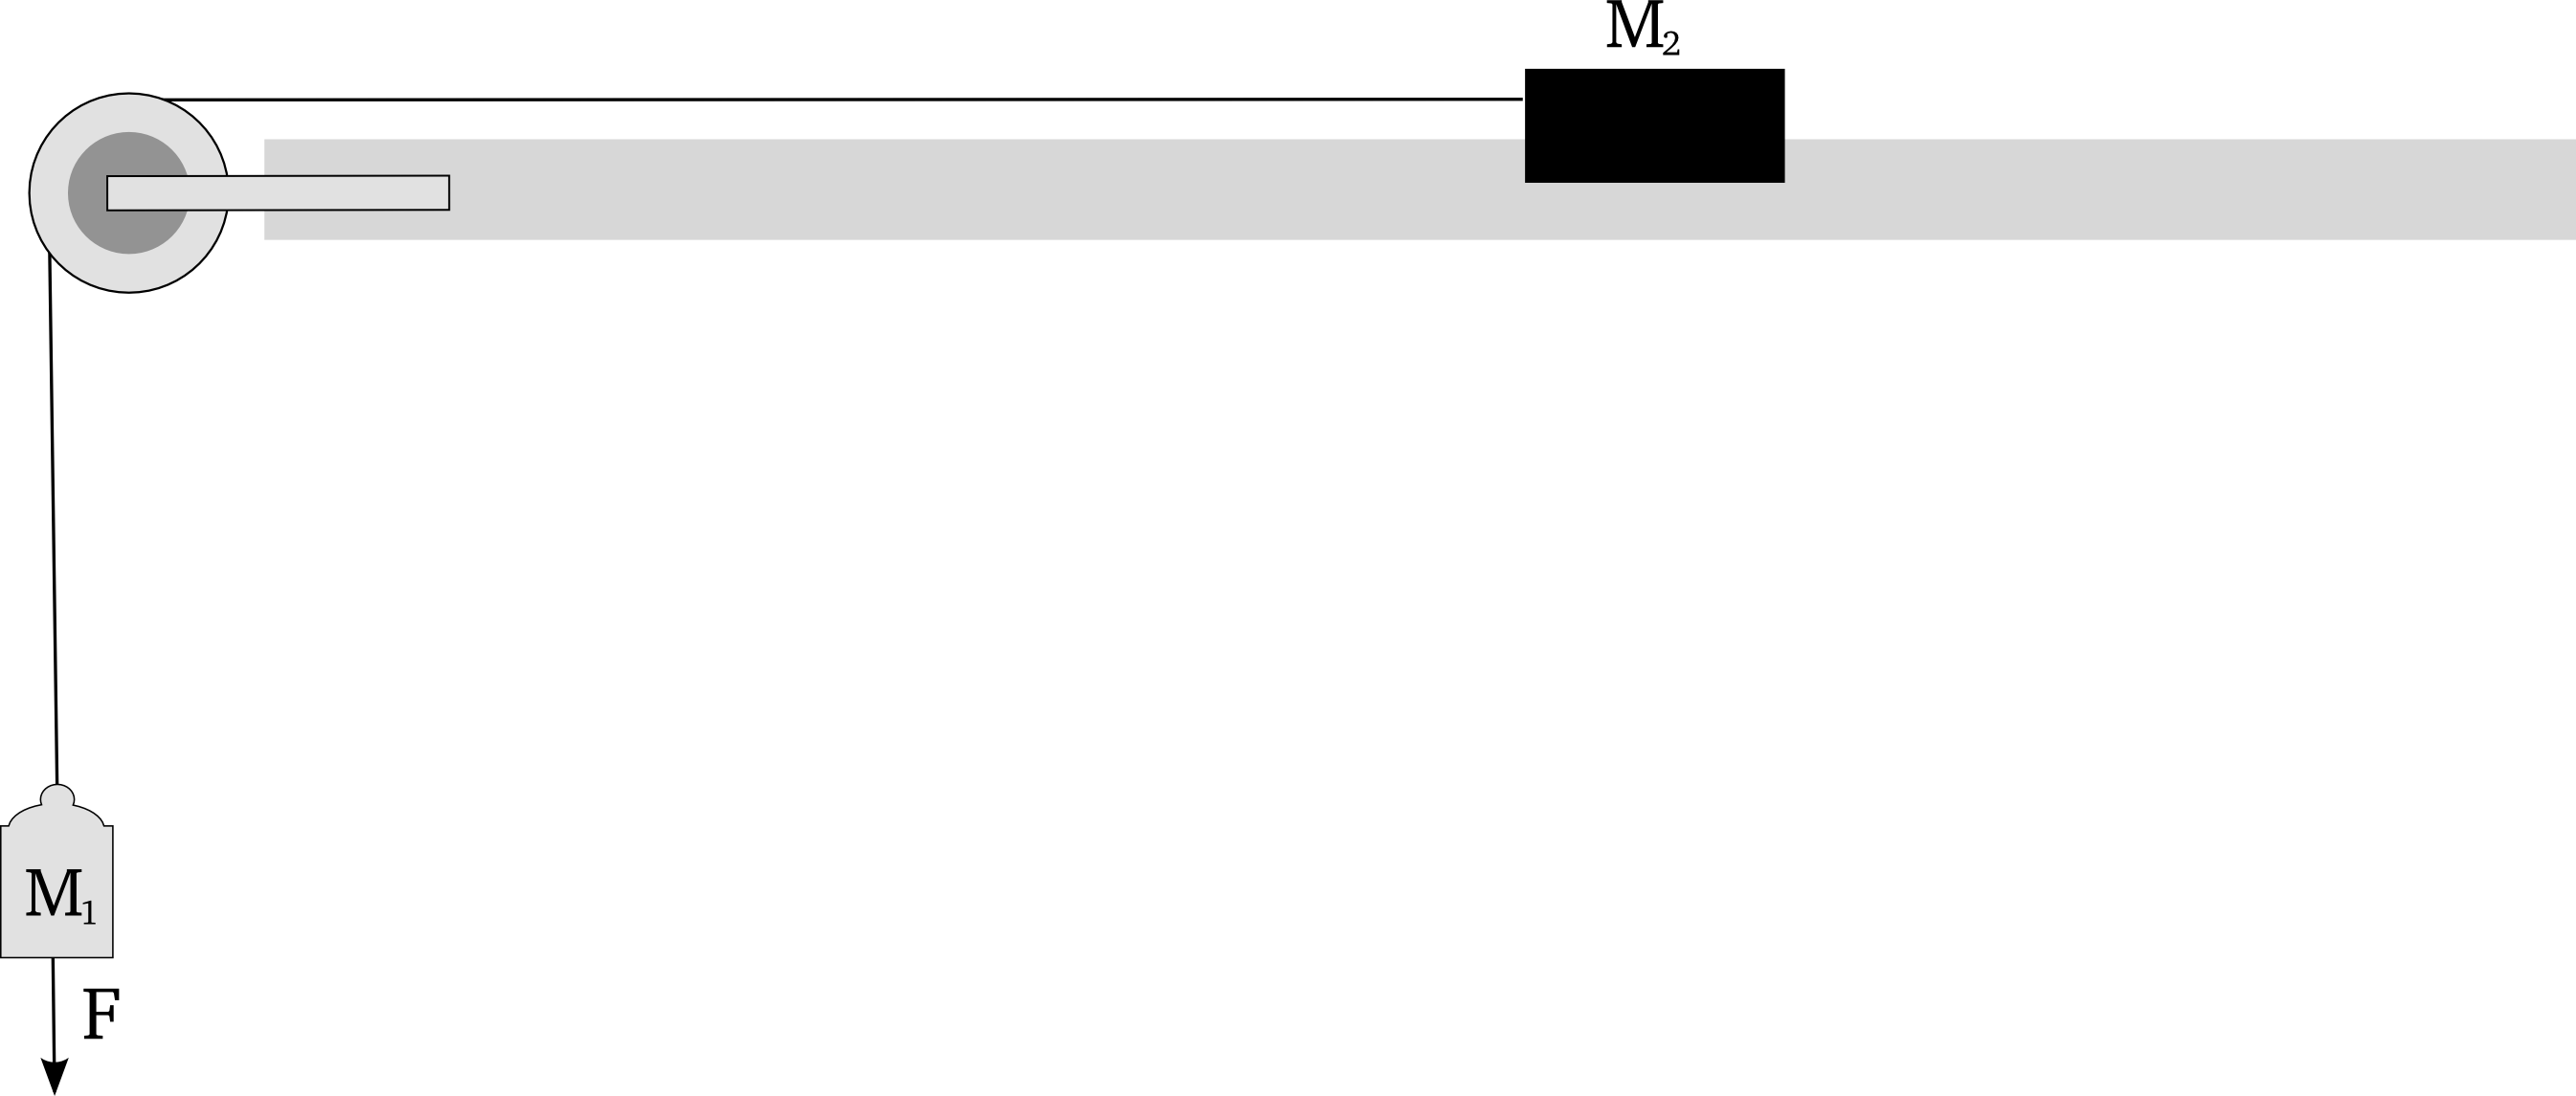
\includegraphics[width=\textwidth]{./Immagini/guidovia.png}
 % guidovia.png: 2691x1145 pixel, 300dpi, 22.78x9.69 cm, bb=
 \caption{Guidovia a cuscino d'aria per la verifica della seconda legge di Newton}
 \label{fig:guidovia}
\end{figure}
Nel primo esperimento utilizzeremo la rotaia a cuscino d'aria ed una forza costante per verificare la validità della seconda legge di Newton. Facendo riferimento alla figura [\ref{fig:guidovia}] la forza costante $\mathbf{F}$ è rappresentata dalla forza peso sulla massa $M_1$, sul corpo composto dalle masse $M_1$ ed $M_2$ collegate da un filo di massa trascurabile ed inestensibile agisce quindi una forza di modulo $F=M_1 g$. Tramite il sensore di moto dovremmo quindi misurare una accelerazione in modulo:
\begin{equation}
 a=\frac{F}{M_1+M_2}
\end{equation}
In laboratorio effettueremo varie misure di accelerazione variando di volta in volta la massa del carrello fluttuante sulla guidovia a cuscino d'aria. Dopo aver effettuato le misurazioni dovrete riportare in una tabella, massa e corrispondente accelerazione del carrello.

\section{L'attrito radente}
L'esperienza quotidiana sembra contraddire la prima legge di Newton, se infatti lanciamo un oggetto sul tavolo questo dopo un breve lasso di tempo si ferma e non continua il suo moto con velocità costante, come invece ci suggerisce la legge di inerzia.
Per spiegare questo fenomeno dobbiamo supporre che tra l'oggetto e il tavolo ci sia una forza (nota come forza d'attrito) che produce la decelerazione osservata. Si è scoperto sperimentalmente che il modulo di tale forza è:
\begin{equation}
 F_a=\mu F_n
\end{equation}
dove $F_n$ è il modulo della forza normale alla direzione dello spostamento e $\mu$ è il coefficiente d'attrito. È possibile misurare un coefficiente d'attrito statico $\mu_s$ quando il corpo è fermo ed un coefficiente d'attrito dinamico $\mu_d$ quando il corpo è in moto. 
In laboratorio utilizzeremo il sensore di forza per determinare il coefficiente di attrito statico per varie superfici e cercheremo di provare come questo sia indipendente da $F_n$

\section{Misura di g}


Per la misura di $g$ utilizzeremo due sensori a infrarossi come in figura [\ref{fig:gravita_1}]
\begin{figure}[H]
 \centering
 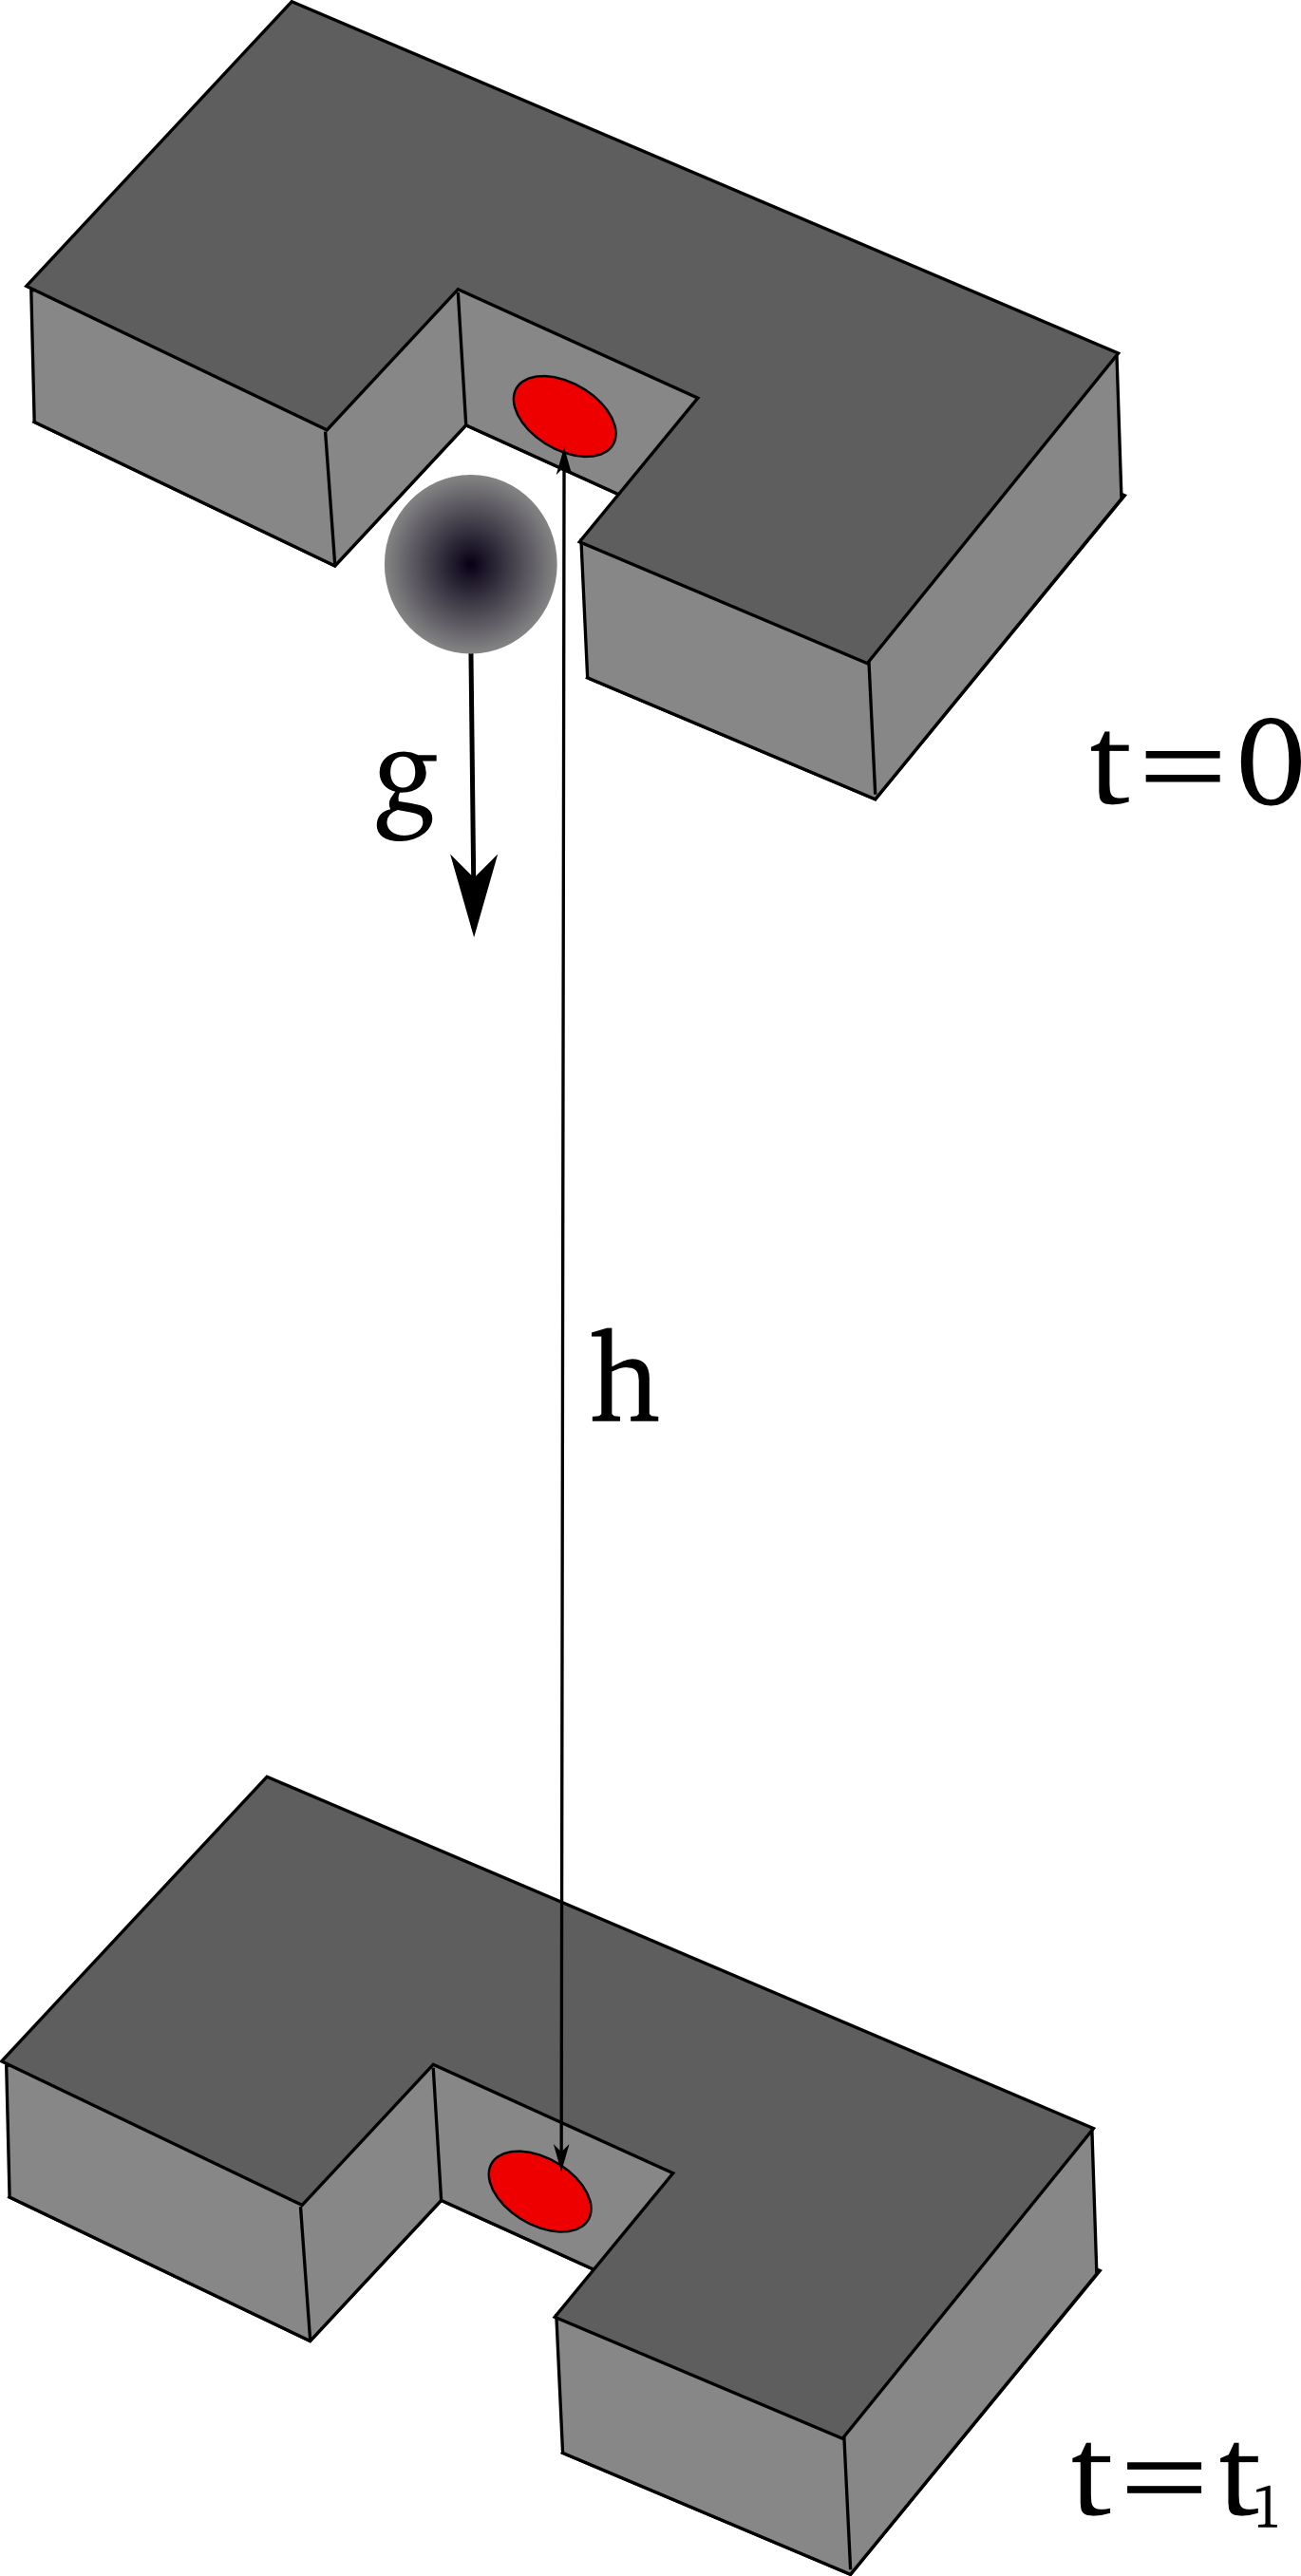
\includegraphics[width=0.3\textwidth]{./Immagini/gravita.png}
 % gravita.png: 1370x2713 pixel, 300dpi, 11.60x22.97 cm, bb=
 \caption{Sensori ad infrarossi per la determinazione del tempo di caduta.}
 \label{fig:gravita_1}
\end{figure}
il cronometro collegato ai rilevatori ad infrarossi ci darà il tempo di caduta, applicando la nota relazione cinematica per il moto uniformemente accelerato:
\begin{equation}
 g=\frac{2s}{t^2}
\end{equation}
possiamo ottenere una stima dell'accelerazione di gravità.
\section{Il pendolo semplice}
Durante la sessione di laboratorio misureremo il periodo di un pendolo semplice da cui dedurremo il valore dell'accelerazione di gravità. Ricordiamo che nell'approssimazione di piccole oscillazioni, ovvero se l'angolo $\theta$ con la verticale è inferiore a 5° il periodo del pendolo è indipendente dall'ampiezza dell'oscillazione e vale:
\begin{equation}
 T=2\pi\sqrt{\frac{L}{g}}
\end{equation}
dove $L$ è la lunghezza del braccio del pendolo e $g$ l'accelerazione di gravità l'equazione del moto del pendolo. Ricordiamo l'equazione del moto del pendolo semplice:
\begin{equation}
 \theta=\theta_0\sin(\omega_0 t+\varphi)
\end{equation}
dove $\omega_0$ è la pulsazione:
\begin{equation}
 \omega_0=\sqrt{\frac{g}{L}}
\end{equation}
e $\varphi$ è la fase del moto. Si può dimostrare che nel caso di grandi oscillazioni la pulsazione $\omega$ vale:
\begin{equation}
 \omega=\omega_0\left[1+\frac 1 4 \sin^2\left( \frac{\theta_0}{2}\right)+\frac{9}{64}\sin^4\left( \frac{\theta_0}{2}\right)+...  \right]^{-1}
\end{equation}
ed il periodo:
\begin{equation}
T=2\pi\sqrt{\frac{L}{g}}\left[1+\frac 1 4 \sin^2\left( \frac{\theta_0}{2}\right)+\frac{9}{64}\sin^4\left( \frac{\theta_0}{2}\right)+...  \right]
\end{equation}
nelle formule precedenti $\theta_0$ è la massima ampiezza di oscillazione.

Le formule precedenti sono valide solo nel caso ideale in cui la massa oscillante è puntiforme e la corda di sospensione è priva di massa.


\section{Il paranco}

Il paranco è una macchina semplice usata fin dall'antichità per amplificare la forza umana. Durante il laboratorio useremo delle carrucole per costruire i paranchi mostrati in figura [\ref{fig:paranco}]. Dovremo tener conto della massa finita delle carrucole sospese che andrà a sommarsi a quella del carico sollevato.
\begin{figure}[H]
 \centering
 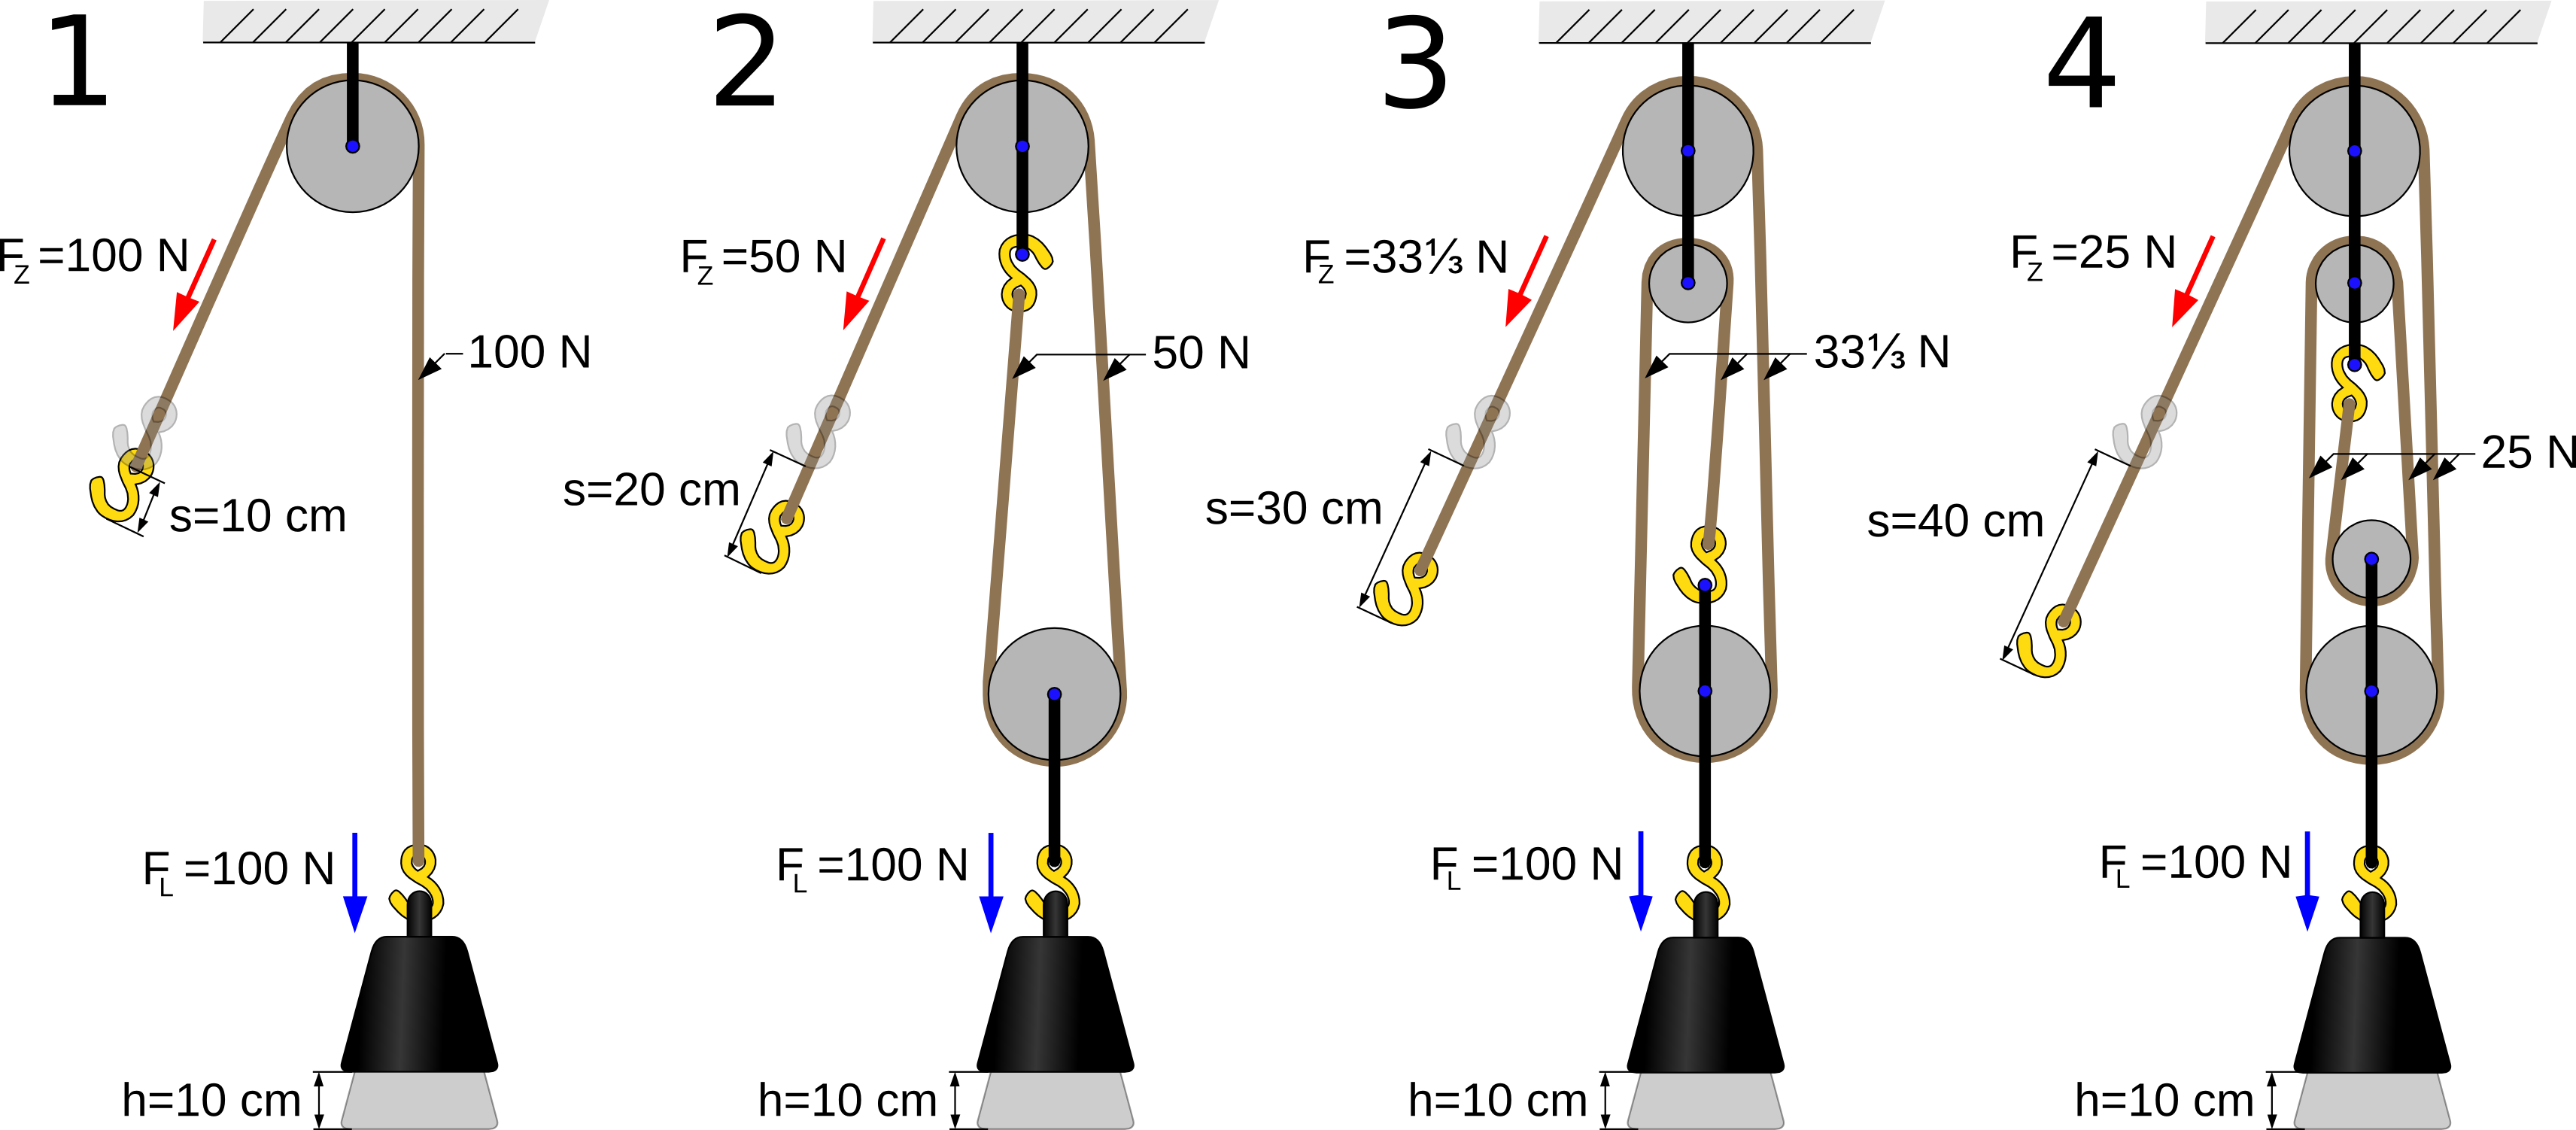
\includegraphics[width=\textwidth]{./Immagini/Four_pulleys.png}
 % Four_pulleys.png: 3424x1502 pixel, 200dpi, 43.47x19.07 cm, bb=
 \caption{Esempi di paranco}
 \label{fig:paranco}
\end{figure}



\section{Moto di un grave incatenato}

In questa esperienza vedremo come il moto di un grave incatenato si discosta da quello di un corpo in caduta libera. Tramite un filmato ad alta velocità misureremo lo spostamento verticale della massa collegata alla catena, quindi dall'analisi delle posizioni dell'oggetto calcoleremo la velocità e l'accelerazione e vedremo come queste si discostano da quelle di una massa in caduta libera.
\begin{figure}[H]
 \centering
 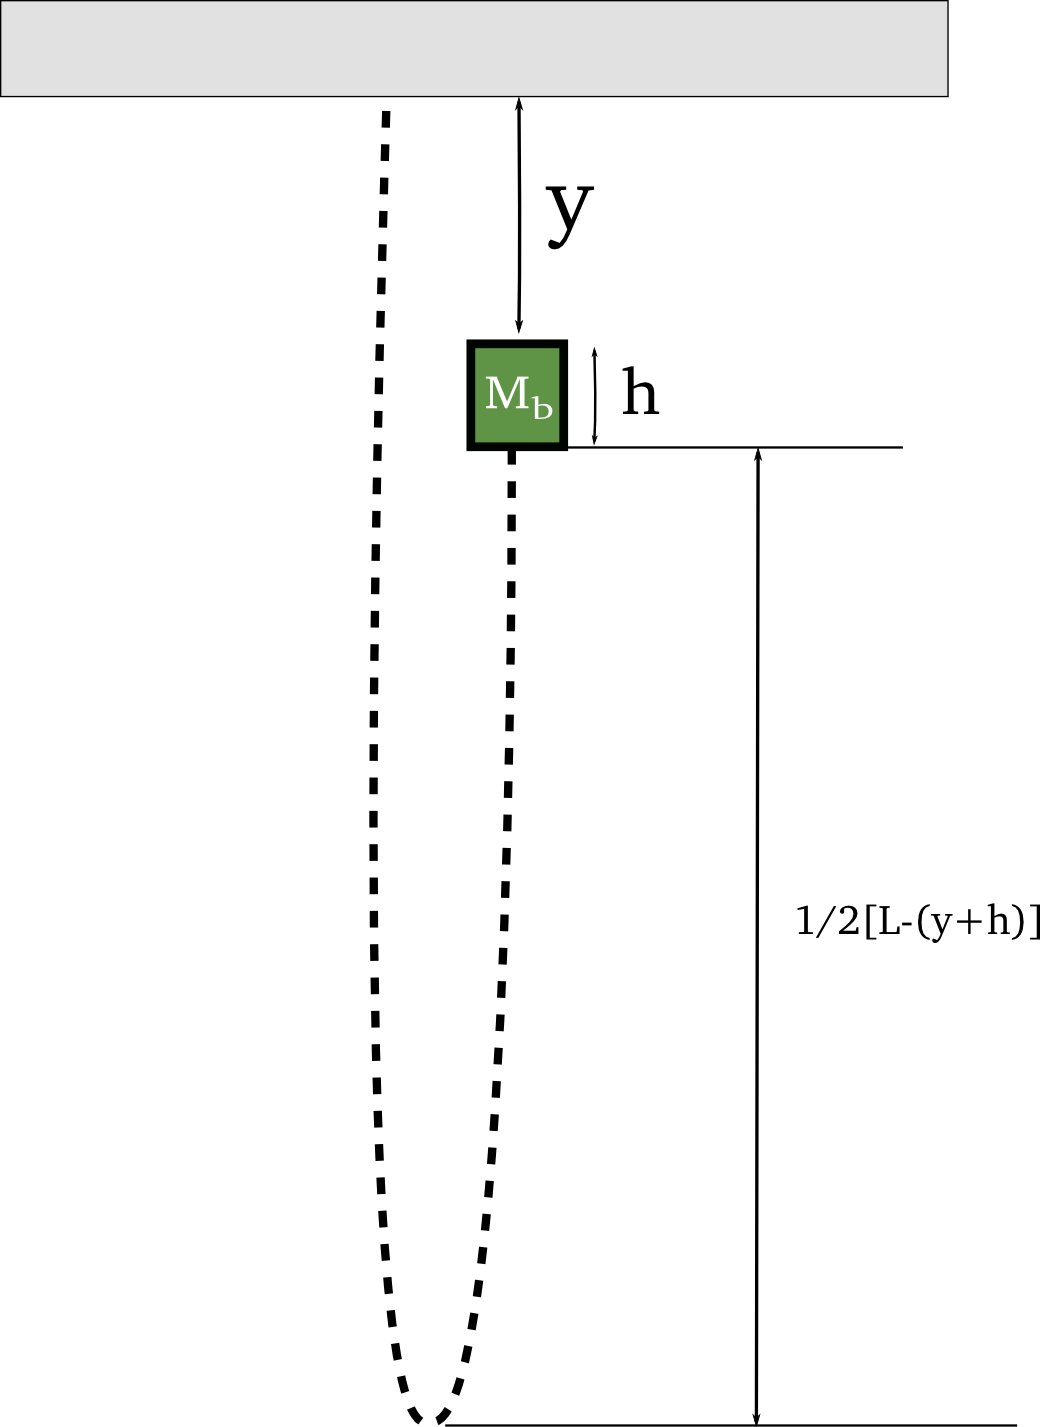
\includegraphics[width=0.6\textwidth]{./Immagini/bungiie.png}
 % bungiie.png: 1040x1427 pixel, 300dpi, 8.81x12.08 cm, bb=0 0 250 342
 \caption{Esperimento per la determinazione del moto di un grave incatenato}
 \label{fig:moto_incatenato}
\end{figure}

Possiamo meglio comprendere questo comportamento notando che per fermare gli anelli della catena in prossimità del punto di inversione deve essere esercitata una forza verso l'alto (sia dalla parte di catena fissata al soffitto che dalla parte di catena in caduta libera) per il terzo principio della dinamica l'elemento di catena in fase di rallentamento eserciterà una forza uguale ed opposta sulla parte sospesa e sulla parte in caduta. La massa della catena e del blocco in fase di caduta possono essere espresse come:
\begin{equation}
 M(t)=M_b+\frac{1}{2}(L-y(t))\lambda
\end{equation}

mentre la forza esercitata dall'elemento frenato sul sistema in caduta può essere espressa come:
\begin{equation}
 F_T=\frac{\lambda}{4}v^2(t)
\end{equation}
Utilizzando queste informazioni è possibile scrivere l'equazione del moto del sistema massa+catena,\footnote{L'equazione del moto risulta essere: 
\begin{equation}
 M(t)g=\frac 1 2 \dot{M}(t)v(t)+M(t)a(t)
\end{equation}
}
e ricavare l'accelerazione e la velocità del sistema ad una data quota, sfortunatamente non è possibile scrivere la dipendenza temporale di accelerazione e velocità in termini di funzioni elementari. In laboratorio cercheremo di ottenere sperimentalmente la dipendenza temporale di velocità ed accelerazione che confronteremo con quelle del moto di caduta libera.



\end{document}
